\tikzset{every picture/.style={line width=0.75pt}} %set default line width to 0.75pt

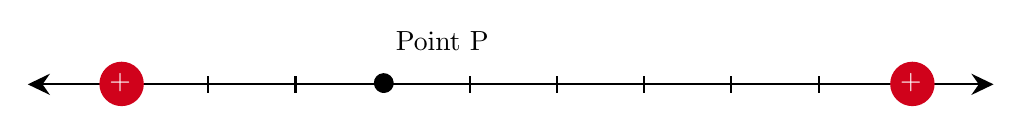
\begin{tikzpicture}[x=0.75pt,y=0.75pt,yscale=-1,xscale=1]
%uncomment if require: \path (0,300); %set diagram left start at 0, and has height of 300

%Straight Lines [id:da8779501834591339]
    \draw    (103,108) -- (562.3,108) (145,104) -- (145,112)(187,104) -- (187,112)(229,104) -- (229,112)(271,104) -- (271,112)(313,104) -- (313,112)(355,104) -- (355,112)(397,104) -- (397,112)(439,104) -- (439,112)(481,104) -- (481,112)(523,104) -- (523,112) ;
    \draw [shift={(565.3,108)}, rotate = 180] [fill={rgb, 255:red, 0; green, 0; blue, 0 }  ][line width=0.08]  [draw opacity=0] (10.72,-5.15) -- (0,0) -- (10.72,5.15) -- (7.12,0) -- cycle ;
    \draw [shift={(100,108)}, rotate = 0] [fill={rgb, 255:red, 0; green, 0; blue, 0 }  ][line width=0.08]  [draw opacity=0] (10.72,-5.15) -- (0,0) -- (10.72,5.15) -- (7.12,0) -- cycle ;
%Shape: Circle [id:dp23414922521798065]
    \draw  [color={rgb, 255:red, 208; green, 2; blue, 27 }  ,draw opacity=1 ][fill={rgb, 255:red, 208; green, 2; blue, 27 }  ,fill opacity=1 ] (135,107.8) .. controls (135,102.17) and (139.57,97.6) .. (145.2,97.6) .. controls (150.83,97.6) and (155.4,102.17) .. (155.4,107.8) .. controls (155.4,113.43) and (150.83,118) .. (145.2,118) .. controls (139.57,118) and (135,113.43) .. (135,107.8) -- cycle ;
%Shape: Circle [id:dp46731974346357785]
    \draw  [color={rgb, 255:red, 208; green, 2; blue, 27 }  ,draw opacity=1 ][fill={rgb, 255:red, 208; green, 2; blue, 27 }  ,fill opacity=1 ] (516,107.8) .. controls (516,102.17) and (520.57,97.6) .. (526.2,97.6) .. controls (531.83,97.6) and (536.4,102.17) .. (536.4,107.8) .. controls (536.4,113.43) and (531.83,118) .. (526.2,118) .. controls (520.57,118) and (516,113.43) .. (516,107.8) -- cycle ;
%Shape: Circle [id:dp6093593677654638]
    \draw  [fill={rgb, 255:red, 0; green, 0; blue, 0 }  ,fill opacity=1 ] (267.24,107.58) .. controls (267.11,105.22) and (268.92,103.22) .. (271.28,103.11) .. controls (273.64,103.01) and (275.67,104.84) .. (275.8,107.2) .. controls (275.93,109.56) and (274.13,111.56) .. (271.76,111.67) .. controls (269.4,111.77) and (267.38,109.94) .. (267.24,107.58) -- cycle ;

% Text Node
    \draw (137+.8,96+5) node [anchor=north west][inner sep=0.75pt]   [align=left] {\textcolor[rgb]{1,1,1}{+}};
% Text Node
    \draw (518+.8,96+5) node [anchor=north west][inner sep=0.75pt]   [align=left] {\textcolor[rgb]{1,1,1}{+}};
% Text Node
    \draw (275.8,81.2) node [anchor=north west][inner sep=0.75pt]   [align=left] {Point P};


\end{tikzpicture}